In this chapter, we describe relevant background information for this work. We define code quality, describe the clean code principles and explain the relation between clean code and code quality. We then introduce different techniques for static code analysis and define a taxonomy based on different complexity levels of automated checker for clean code violations. Afterwards, we introduce quantitative metrics to measure the code quality and their useability to measure clean code violations. We conclude with an overview of related work in the form of tools for code quality analysis and in academic research.

\section{Code Quality}\label{sec:code_quality}
Before defining code quality, we define software quality. According to ISO/IEC 25010:2011 standard, software quality describes the degree \enquote{to which a product or system can be used by specific users to meet their needs to achieve specific goals with effectiveness, efficiency, freedom from risk and satisfaction in specific contexts of use}~\cite{iso_central_secretary_isoiec_2011-1}. Software is written with source code, so the quality of the source code reflects the software quality on the implementation level. Additionally, factors such as software architecture and chosen technologies influence the overall software quality on the system and conceptual level.

The standard specifies eight characteristics for software quality~\cite{iso_central_secretary_isoiec_2011-1}. The main influence of source code and its quality is on those four characteristics:
\begin{enumerate}
    \item Reliability
    \item Performance efficiency
    \item Security
    \item Maintainability
\end{enumerate}
Reliability is the ability of a system to run without critical exceptions that would cause the system to crash, become unavailable or result in an inconsistent state. A code with high quality runs without such critical exceptions. Performance efficiency describes an optimal use of the resources like CPU-time, memory or network bandwidth. Well written code with a high quality use the resources efficiently. The security aspect focuses on minimizing possible attack vectors. Software is vulnerable if the source code implements behaviour in an unsafe way. A code with high quality would implement its functionality with a focus on the security aspect. 

Software maintainability consists mainly of those activities that involve changing source code:
\begin{enumerate}
    \item Adding code for new features
    \item Implementing changed requirements by modifying code
    \item Fixing bugs to ensure correct functionality of the software
\end{enumerate}
The importance of good maintainability of source code is based on the associated cost. 
For project planning, different sources suggest, that project manager should estimate 66\% or even 75\% of the total software costs for maintenance~\cite{yip_software_1994, galorath_accurately_2019}. A recent study from 2018, conducted by Stripe and Harris Poll highlights that developers spent 42\% of their work time maintaining code~\cite{stripe_developer_2018}. Increasing the effectiveness of maintaining code is consequently cost-relevant. The easiness of code changeability due to code quality becomes a business-critical requirement and can positively impact the maintainability in the following ways~\cite{baggen_standardized_2012}:
\begin{enumerate}
    \item Well-written code makes it easy to determine the location and the way source code has to be changed.
    \item A developer can implement changes more efficient in good code.
    \item Easy to understand code can prevent unexpected side-effects and bugs when applying a change.
    \item Changes can be validated easier. 
\end{enumerate}

The application of agile software development methodologies like Scrum is another important contributor for code to be changeable with the least possible effort. Scrum is an agile software development practice of building software in increments while having a running software at the end of each increment. One of the advantages is the adaptability of this model to changing requirements, since, with the end of each increment, a requirement change can be implemented~\cite{schwaber_agile_2002}. 

To sum up, code quality is part of the overall software quality on the implementation level. It contributes to several characteristics of software quality, with the most important one being the maintainability. A good code quality allows efficient changes and therefore, high maintainability.

\section{Clean Code}\label{sec:clean_code}
In \Cref{sec:code_quality}, we defined the terminology of software and code quality. The clean code concept describes rules and is coined by Robert C. Martin in his book \enquote{Clean Code: A Handbook of Agile Software Craftsmanship}~\cite{martin_clean_2009}. Those rules should ensure readability and understandability for the developers. With understandability and readability, the changeability and in turn the maintainability of code is impacted.   

The author describes clean code principles in the form of practical rules. Those practical rules shall result in clean code that is easy to understand and read. Chaotic code, by contrast, is harder to read and understand. The author argues, developers produce chaotic code in a conflict between deadline pressure and the necessary effort to make code more intuitive and follow clean code principles~\cite{martin_clean_2009}. The former pressure is created by deadlines that focus on the visible output like the functionality of the program, whereas the latter is not directly visible in the final product. If the success criteria are solely based on the visible output, the code quality may suffer by fast-to-write chaotic code. This behaviour is shortsighted since an accumulation of chaotic code reduces productivity over time. A larger system with chaotic code will slow down later modifications or additions of code. With the costs associated with maintainability as described in \Cref{sec:code_quality}, reducing the maintenance effort is a logical step. With the clean code principles, developers can read and understand code in a more intuitive way, and the described costs of chaotic code will decrease~\cite{martin_clean_2009}.

The following sections explain the clean code guidelines, as described by Robert C. Martin~\cite{martin_clean_2009}. First, we describe rules for naming and functions. Then we recap rules regarding comments, data structures and objects. Finally, we conclude with suggestions for classes and error handling.

\subsection{Naming}\label{sec:naming}
The naming section covers several rules for naming variables, functions, types and classes.
Good naming can make it easier to read and understand code. \enquote{Good} naming is an opinionated topic; For Robert C. Martin, the key factor of good naming is the descriptiveness of names~\cite{martin_clean_2009}. Descriptive names provide the reader with enough information to understand what a variable stores or what a function computes. Abbreviations or symbolic names like \textit{a1, a2} are not descriptive and do not provide information about the meaning. Using symbolic names for mathematical expressions could be an exception to the rule if the naming mirrors the expression.

To come up with a descriptive name, it is helpful to include a verb or verb expression for function names, because functions express an action. For class names, a noun emphasises the object character of the class.

Another valuable property of a name is an easy pronunciation since it is easier to read and to talk about the code with other developers. For reading, the pronunciation improves subvocalization\footnote{the internal speech when reading}. Non-dictionary words or unusual abbreviations are harder to pronounce. Consequently, it is useful to make longer but descriptive and pronounceable names, especially since the autocomplete feature of IDEs will free the developer from typing the long name. Additionally, searching for long names works better than for short names, because long names are more likely to be unambiguous compared to shorter names. Acceptable exceptions to this rule are short variables in a small scope (e.g. variable \textit{i} in a loop), but using \textit{i} in a large scope could be ambiguous and troublesome for searching and understanding.


\subsection{Functions}\label{sec:functions}
This chapter describes several rules regarding functions, that Robert C. Martin charactericse~\cite{martin_clean_2009}. 

First, functions should be small in length. Exceeding 20 lines should not be necessary in most cases. If a function is small, it can be read more easily and without scrolling. 

Second, inside a function, if-, else- and while-statements should contain a function call for the body. Additionally, the rule of descriptive naming can apply to the condition of the if statement: If the condition becomes hard to understand, a function call can simplify the understanding of the condition. With a descriptive naming, a function call documents the condition and body in a concise and readable way. In \Cref{lst:function_method_call}, reading a condition with function calls does not require the reader to decrypt the logical expression. This can also save additional comments that explain the meaning of the condition. Furthermore, since the body also contains a function call, it is fast to understand the cause-effect relation of the if expression. 

\begin{lstlisting}[float=t , language=Python, label=lst:function_method_call, caption={Sample for using functions with if-statements with the increased documentary value of the cause-effect relationship.}]
if person.is_authorized():
    modify_data()
else:
    redirect_to_login()
\end{lstlisting}


Third, functions should fulfil one purpose. Since functions may have to call several functions subsequently to perform the necessary computation, Robert C. Martin expands the rule that functions should only operate on one abstraction level~\cite{martin_clean_2009}. This would result in the following structure:
Functions with a low abstraction level handle data access and manipulation, e.g. string manipulation. Functions on a middle abstraction layer orchestrate the low-level operations. On the next higher level, the mid-level functions are orchestrated. Following this structure, a function has one purpose on the low level and one orchestration function on a higher abstraction layer. 

Fourth, the number of function arguments should be three or lower. With many function arguments, it becomes harder to call a function. Simultaneously, testing becomes harder, especially if all argument combinations should be tested. Functions with none or one argument simplify testing. Since testing can reveal bugs, testable code is crucial for reducing the number of bugs.
If a function requires more arguments, it may be advisable to bundle those in a config object to pass multiple arguments as one. With a config object, arguments can be logically grouped that would help the reader to understand arguments. 

Fifth, side-effects in a function body should be avoided. Side-effects happen if a function modifies a variable outside its scope without explicitly mentioning this in the function name. This leads to dependencies between the functions that are not obvious to a developer who checks the signature, i.e. the name, input arguments and return type, to use the function. To spot a side-effect, the developer would have to read through the function, although reading the signature should be enough to use the function. With side-effects, the function behaves unexpected, and time-consuming mistakes are the consequence. Especially side-effects that initialise other objects result in a time-dependency that is hard to identify and could be overseen at all.

The next rule forbids the returning of error codes and suggests raising an exception if the programming language supports it. Raising an exception allows better separation between application logic and error handling code since the error code checking interrupts the reading flow of code. Additionally, catching a raised exception is separated from the logic for a non-error execution and can be separated into an additional function for an even cleaner structure. \Cref{lst:error_catching} shows an implementation of a simple function with exception raising and error code return in the \texttt{database.read\_all\_users()} method. The former error handling shows the separation between the application logic and the error handling logic, whereas the error handling in the latter interrupts the reading flow of the code.

\begin{lstlisting}[float=t , language=Python, label=lst:error_catching, caption={Sample listing for error handling with try and except statements vs error codes.}]
def query_all_admins():
    try:
        all_users = database.read_all_users()
        admins = [user for user in all_users if user.is_admin]
        return admins
    except DatabaseError as error:
        print("Database error", error)

def query_all_admins():
    all_users = database.read_all_users()
    if all_users == -1: #-1 is database error
        print("Database error code -1")
    else:
        admins = [user for user in all_users if user.is_admin]
        return admins
\end{lstlisting}


Last, the important principle for software engineering applies directly to functions: \enquote{Do not repeat yourself}~\cite{haoyu_basic_2012}. Repeated code is dangerous and chaotic since it requires changes in multiple locations if it has to be modified. This makes duplicated code very prone to copy and paste errors and small mistakes that may not be obvious during development but will lead to a fatal crash at runtime. Code clone detection is an active research field, especially for finding semantic clones without syntactic similarity. For instance, Büch and Andrzejak suggest an AST-based recursive neural network~\cite{buch_learning-based_2019} and Saini et al. present an approach that can even detect duplications with just minor syntactic similarities~\cite{saini_oreo_2018}.

\subsection{Comments}
Comments are part of every programming language and can play an important role in code quality. Subjectively good comments clarify the meaning of the code and help to understand the code. However, comments can become outdated and wrong or provide useless information~\cite{martin_clean_2009}. In a perfect world, the programming language and the programmer would be expressive enough that commenting is not required for clarity. Following the clean code guidelines for naming and functions makes many descriptive comments obsolete, since the function description is encoded in the function name.

Comments will not help to turn chaotic code into clean code. If a developer explains a line of code by a comment, it is often more helpful to call a function with a descriptive name to replace the comment. Since comments are not part of the program logic, if the explaining comment is not updated with the code, the comment gives misinformation to the reader like described before.

In brief, before writing a comment, the developer should think about expressing the same in code. Robert C. Martin gives some exceptions for situations, where comments can be helpful or necessary~\cite{martin_clean_2009}:

\begin{description}
    \item[Legal notes:] Legal notes like copyright or license information and author mentions may be necessary. Although they should be short and link to an external licensing document in full extent.
    \item[Explaining comments:] Some explaining comments can be helpful and are not easy to encode in regular code. For instance, an explanation of a complex regular expression may be too complicated for a function name, and a comment provides the space for a sufficient explanation. This increase the readability since the developer does not need to interpret the regular expression manually.
    \item[Intention:] Explaining an intention which does not become evident by reading the source code might also be a valid use-case for a comment. 
    \item[Warning for consequences:] Some parts of the code can have extraordinary consequences like not being thread-safe or using many system resources. A warning can spare a developer from having trouble when using the function.
    \item[Emphasise :] A comment to emphasise the importance of a seemingly unimportant part of the code prevents breaking modifications of the code. 
\end{description}

\subsection{Data Structures and Objects}
This chapter describes the rules of data structures and objects. Both store data but the way this data get exposed differ. Objects hide data behind abstractions and have functions that work with these data. Data structures expose the data and do not provide functionality. 

For objects, I. Holland defined the Law of Demeter (LoD)~\cite{lieberherr_assuring_1989}.
In object-oriented programming, a method $m$ of an object $O$ may only call methods of the following components:
\begin{itemize}
    \item the object $O$ itself
    \item the parameters of the method
    \item objects that are created within $m$'s scope
    \item instance variables of $O$
\end{itemize}
In other words, the object $O$ only calls methods on direct \enquote{neighbours} or on itself. The object does not call a method of its neighbour to subsequently call a method on the returned object from the neighbour. By restricting the allowed method calls outside the object itself to direct \enquote{neighbours}, the dependencies between objects are reduced, and the modularity increased. As a consequence, changing methods only affects the direct neighbours and not objects in potentially different parts of the software. 
\Cref{fig:LoD} shows an example for the LoD. In the method \texttt{test}, a function call on \texttt{B} returns a reference to \texttt{C}. Since \texttt{C} is not a direct neighboor of \texttt{A}, the function call violates the LoD. The modularity of objects suffer, since a change of the method \texttt{do\_something()} would require changes in object \texttt{A}. This close coupling of an \texttt{A} and \texttt{C} is circumvented with a method \texttt{do\_something\_on\_C} that wraps the functionality of \texttt{C}, so a change in \texttt{C} would only require a change in B. With that common layer, \texttt{A} and \texttt{C} are decoupled. Object \textit{A} in this case does not know how the certain functionality is performed and it does not matter.  
Bad code practice like the violation of the LoD in \Cref{fig:LoD} is called a train wreck since subsequent method calls look like multiple train carriages. The described wrapping function can improve such train wrecks.

\begin{figure}
\begin{tabular}{p{0.45\textwidth}p{0.45\textwidth}}
    \begin{minipage}{0.45\textwidth}
        \centering
    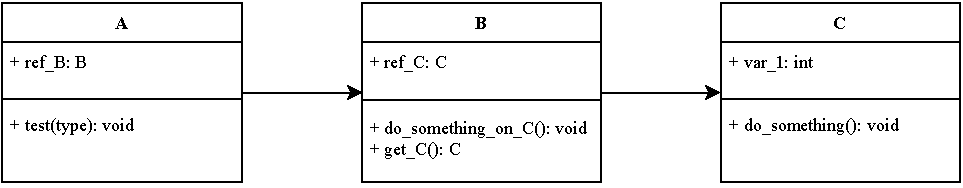
\includegraphics[width=\linewidth]{img/Background/LawOfDemeterUML.pdf}
    \label{fig:background_control_flow_graph_image}
    \end{minipage}
&
\begin{minipage}[c]{0.45\textwidth}
\centering
\begin{lstlisting}[language=Python, label=lst:background_control_flow_graph_listing]
def test():
    #violation of LoD
    self.B.get_C().do_something()

    #no violation of LoD
    self.B.do_something_on_C()
\end{lstlisting}
\end{minipage}
\end{tabular}
\caption{A sample illustration of the Law of Demeter. The figure on the left shows a class diagram for the classes \textit{A}, \textit{B} and \textit{C}. The listing on the right shows the implementation of the \textit{test} method of class \textit{A}. }
\label{fig:LoD}
\end{figure}



Data structures are often used as Data Transfer Objects (DTO) to communicate with other processes or services. These objects do not contain any functions; instead, they only have accessible member variables. Specializations of DTOs are Active Records that contain additional methods for data storage. They are used to represent a data source like a database. For DTOs and Active Records, it is a bad practice to insert business logic into these objects~\cite{martin_clean_2009}. With business logic, the data structure becomes a hybrid between an object and a data structure. It becomes unclear if the purpose of a hybrid is to store data or to expose methods to modify those data in a controlled way. Without the clear purpose of the object or data structure, it becomes harder to understand for developers.


\subsection{Classes}\label{sec:classes}
For classes, the clean code principles describe multiple rules that improve the readability and understandability of classes.

The first rule specifies the recommended size of a class. Unlike counting lines as for functions, the size of a class is the number of responsibilities. A responsibility of a class can be manipulating data or writing data to a file. A single responsibility per class is described as Single-Responsibility-Principle and offers several advantages: First, the naming can reflect this responsibility, so the class functionality is easy to understand.
Second, changing one functionality should only require changes in the one class that is responsible for this specific function. And last, we can reuse the class in different projects if we need that functionality. If the class fulfilled two responsibilities, we would have to remove the unnecessary functionality before reusing the class in a different project. Reaching back to the examples of one responsibility being data manipulation and one is writing data to a file, reusing the latter functionality would require us to strip out the data manipulation.
The Single-Responsibility-Principle leads to a system of many small classes with one, clearly defined responsibility.

The second rule recommends classes to have high cohesion. The ohesion is high if a method manipulates many instance variables. If all methods of a class manipulate all instance variables, the class has its peak cohesion. With a high cohesion, the methods and the class are a logical unit. A low cohesion indicates to split the class into multiple classes since the methods are not a logical unit. As a result of splitting classes into smaller logical units, they will more likely comply with the Single-Responsibility-Principle.

The last rule provides a guideline on how to handle internal or third-party class dependencies. If a dependency changes, the class depending on it should not change. To accomplish this decoupling from the implementation of a dependency, classes should not depend on the dependency directly but instead on an abstract class (or interface). That abstract class describes the concept of the dependency that is unlikely to change. For example, for a database dependency, the abstract class defines the concepts of storing and retrieving an entry. For the specific database, a specific class implements the abstract class or interface and provides the functionality. Changing the database only changes the implementation in the specific class but not the concept. Therefore, there is no need to modify a class that depends on the concepts from the abstract class. This isolation of dependencies is especially useful if the dependencies are not under the developer's control and may be changed any time by a third party. The abstraction is also valuable for testing since the dependency can be replaced by a so-called mock class that only simulates the behaviour. This allows testing to be independent of the dependency and to locate potential errors in the own system or the dependency.

\subsection{Exception Handling}\label{sec:background:returning_none_and_error_handling}
This chapter covers clean code rules for error handling. The following ways are methods for handling errors:
First, a function can return an error code if some exception occurred. The function caller has to check for the error code and act accordingly. Second, some programming languages support the concept of throwing and catching an exception. And last, a function can return a null value to indicate the execution failure. 

In section \Cref{sec:functions}, we described the clean code rule that prefers throwing an exception over returning an error code. The supporting argument of Robert C. Martin is the better separation between application logic and error handling~\cite{martin_clean_2009}. Error codes have to be checked immediately, so the error checking interrupts the code for the application logic. By throwing and catching errors, the error handling can be completely extracted into a sperate function and can be removed from the main application logic. Furthermore, the try-catch block enforces transactional behaviour. At the end of either the try or the catch block, the application should be in a consistent state. Error codes hide this explicit transactional behaviour. 

Notwithstanding the clean code rules, Go as more recent programming language\footnote{designed in 2007 as a response to problems with C++, Java and Python~\cite{noauthor_go_nodate}} returns explicit error types instead of throwing an exception. This was designed to \enquote{encourage you to explicitly check for errors where they occur}, instead of \enquote{throwing exceptions and sometimes catching them}~\cite{gerrand_error_2011}.   
So the practical application of the clean code rule for throwing exception depends on the design of the programming language.

The third method of error handling is returning a null value. Instead of checking for a specific error code, the caller would check for a null return value. If a developer misses the check, the program will terminate with an unhandled NullPointerException at runtime. Tony Hoare introduced the null reference in 1965 and later called it his \enquote{billion-dollar mistake}~\cite{hoare_null_2009}, since it leads to many bugs and security vulnerabilities throughout the decades. Languages like Kotlin are designed with null safety enforced. Kotlin distinguishes between nullable and non-nullable references, with a compiler enforcing null checking~\cite{noauthor_null_nodate}. If a language does not enforce null safety with a compiler, a special case like an empty collection or an optional type can be returned. 
Returning null introduce the same problems like error code handling such as mixing application and error handling logic and is additionally not explicitly marked as an error code. From a function signature, it may not be evident that the return value may be null if the language does not support compile-time checking or optional types. Robert C. Martin describes returning null as a violation of the clean code rules~\cite{martin_clean_2009}. For Python, the null value is named as \texttt{None} and calling a method a \texttt{None} results in an exception. 

Independent of the error handling method is the next rule for error handling with a third-party library. In section \Cref{sec:classes}, we described wrapping dependencies like third-party libraries to decrease the coupling to the dependency. The wrapping concept also applies to error handling, since the wrapper can unify the exceptions, so the application does not check for dependency-specific error types. Changing the dependency requires only a change in the wrapper implementation but not everywhere this wrapper is used. 

\subsection{Additional Rules}
Robert C. Martin describes more rules for system design, multithreading, testing and third-party code~\cite{martin_clean_2009}. 
Additionally, the author describes the concept of code smells. In theory, following these rules seems to lead to clean code. In practice, however, developers tend to violate rules in some situations. A code smell is a code characteristic that could indicate such a violation.

This work will focus on the described rules and implement a detection for some rule violations.

\section{Source Code Analysis}\label{sec:code_analysis}
In order to define and measure code quality, methods for analyzing a program and its source code are necessary.

To analyse source code, different techniques are bundled as static code analysis. A static code analysis gathers information about the structure of the source code and program~\cite{prahofer_static_2017}.

The following provides a non-comprehensive overview of the most important methods for code analysis and representation.
Source code itself is stored as encoded text files. This representation offers no structural information. 

A first processing step is a lexical analysis, also known as tokenization. The tokenization transforms the character stream from the text file into a stream of tokens. This is possible due to the syntactic definition of a programming language, that allows splitting the raw text into typed tokens~\cite{mogensen_introduction_2017}. A token type can be, for instance, a keyword, operator or an identifier.

With the token stream, a parser can build an Abstract Syntax Tree (AST) that represents the abstract structure of the source code.
Since the AST represents the code structure, it is possible to traverse the tree-like data structure to analyse the code structure.

Another method is the control flow analysis. For the control flow analysis, the program has to be represented as a control flow graph. The control flow graph represents possible execution paths in a program and consists of nodes and edges. A node represents a basic block, i.e. a code sequence without branching. A directed edge represent jumps in the control flow; e.g. an if-statement would have two outgoing edges, one for a true condition and one for a condition evaluated as false~\cite{allen_control_1970}

Besides the control flow, it is possible to analyse the data flow in a data flow graph. With the data-flow analysis, it is possible to collect information about the read and write operations to variables. In combination with the control flow graph, the data flow for different control flow can be calculated~\cite{mogensen_introduction_2017}.

Last, a call graph can be computed. A call graph maps all method or function calls starting from the primary method. It allows spotting dependencies between modules~\cite{prahofer_static_2017}.

\section{Clean Code Complexity Levels}\label{sec:cc_complexity_levels}
We described the clean code rules in \Cref{sec:clean_code}. This work focus on the automated checking of clean code rules. Some rules can be checked straightforward with an algorithm, whereas others may be too abstract to be checked in an automated way. In this Section, we want to group the clean code rules into different complexity levels. The complexity levels are based on the complexity of implementing an automated rule checker. 

We define the taxonomy of complexity in three levels, based on the different source code analysis techniques and effort needed:
\begin{description}
    \item[Basic Level] The level of basic complexity covers all rules that can be checked by a single analysis of the text, token stream, or AST of the program.
    \item[Advanced Level] Rules with medium complexity require a control flow, data flow, call graph analysis or more advanced, deterministic analysis techniques. Furthermore, a combination of different analysis methods from the basic complexity level will be categorised as medium complexity. 
    \item[High Level] The high level of complexity covers the clean code rules we assume can not be checked with traditional, deterministic analysis techniques such as those described in \Cref{sec:code_analysis}. For this level, it may be indispensable to use statistical methods like machine learning approaches to create an automated checker. It is important to note that we do not prove that no deterministic algorithm exists. 
\end{description}

Based on these levels, we categorise the clean code rules introduced in \Cref{sec:clean_code}. \Cref{tab:complexity_level_overview} gives an overview of all rules and our assigned complexity level. In the following, we explain the reasoning behind the categorisation for all rules:


\begin{table}[h]
\begin{tabularx}{\textwidth}{XXccc}
\toprule
&     & \multicolumn{3}{c}{Level} \\ \midrule
Category&Rule & Basic  & Advanced  & High \\ \midrule
Naming&Descriptiveness&&& X\\
Naming&Pronunciation&X&X& \\
Naming&Names in Small Scope&&X& \\
Functions&Length&X&&\\
Functions&Conditional Function Calls&X&X& \\
Functions&Purpose&&&X\\
Functions&Levels of Abstraction&&&X\\
Functions&Number of Arguements&X&& \\
Functions&Side-Effects&&X&X\\
Functions&Error Code Detection&&&X \\
Functions&Duplicated Code&&&X \\
Comments&Detecting Necessary Comments&&&X \\
Objects&Law Of Demeter&&X& \\
Objects&Mix with Data Structures&X&& \\
Classes&Single Responsibility&&X&X \\
Classes&Decouple Dependencies&&X& \\
Errors&Return None&X&& \\
\bottomrule
\end{tabularx}
\caption{Categorisation of clean code rules based on our taxonomy for the complexity of automated checkers.}
\label{tab:complexity_level_overview}
\end{table}


For naming, all rules have in common, that an algorithm would have to extract the names of various entities like variables, classes, functions from the source code first. The AST provides the names and entity types they describe. Extracting all names is a matter of walking over the AST. We see this in the basic complexity level.

The first rule in naming is the descriptiveness of names. Assessing the descriptiveness of a name is a problem with a high level of complexity. An algorithm would have to understand the purpose of the source code to determine if the name describes the source code. It is an ongoing research effort to use machine learning on code for different tasks (TODO \url{https://dl.acm.org/doi/abs/10.1145/3212695}). The tasks of code summarisation explore the use of machine learning to generate a natural language description of source code. In a paper from 2018, Alon et al. describe a neural network to represent code as vectors and \enquote{predict a method’s name from the vector representation of its body}~\cite{alon_code2vec_2018}. Based on that and the following research, it may be possible to compare the summarisation result with the chosen name to detect non-descriptive names. Nevertheless, it may be harder to apply such concepts to variable names, since a variable name has less context information compared to the method name with its method body.

The next naming rule covers the easy pronunciation of names. A rule violation would be the use of abbreviations or non-dictionary words in variable names that are hard to pronounce. An approach with a basic level of complexity could be a minimum number of characters for every name. A more advanced approach could utilise naming conventions such as camel case or underscore separated words to extract the single words of a name and compare it with a dictionary. While it would help to prevent spelling mistakes and should ensure pronounceability, a dictionary may not contain all words. Especially with domain-specific words, this could lead to false alarms.

Variable names in a small, local scope are excepted from the rule of pronounceability and thus longer names. To determine the scope of a variable, the data flow analysis could be used. With the analysis, the previous rule could include this exception. Due to the data-flow analysis, we categorise this rule into the advanced level of complexity.



For functions, the clean code principles define multiple rules. 
First, functions should be smaller than 20 lines of code. A checker for this rule could be grouped at the basic level of complexity since the AST contains all the necessary information about the function body. If the metadata such as line number is retained during AST construction, a checker can calculate the lines of code for the function body.

The next rule covers the function call in the condition and body part of a conditional such as an if-statement. An if-statement is represented as a node with a condition, body and an \texttt{else} descendant. An algorithm can scan the AST to check the condition and body nodes of the conditional statement. Such a checker would have a basic level of complexity. Since a function call mainly increases the understandability of more complex conditions, some threshold such as a maximum number of allowed logical sub-expressions could be applied. With this enhancement, an automated checker could be grouped in the advanced level of complexity.

Regarding the purpose of a function, the clean code rules suggest a function to have one purpose and to operate on one abstraction level. Counting the number of purposes requires an understanding of the semantic of the code. Similar understanding would be necessary for the level of abstraction. We argue such a checker would be in the high level of complexity category since the understanding of code could only be achieved with machine learning. The aforementioned research field of code summarization could be beneficial for this task, too. A natural language description of a function may require the model to \enquote{understand} the purpose and task in order to articulate it in natural language. It may be possible to use work in this field to detect functions with multiple purposes or abstraction levels.
 
The rule that limits the number of function arguments is on a basic level of complexity. The AST contains the information about the code structure and therefore, all function arguments. Counting those requires the algorithm to search for function nodes in the AST and count the number of arguments.

The next rule forbids side-effects of a function. Detecting side-effects can be broken down into a two-step process.
First, tracing the data manipulation of functions is at the advanced level of complexity. With a data-flow analysis and call graph, it is possible to check what variables a function manipulates. Second, the classification whether an effect of a function is a side-effect requires an understanding of the intended effect of a function. The intended effect is described in the name. We argue that the understanding of the intended effect is at the high level of complexity. 

The clean code rules discourage the use of error codes to indicate exceptions. If the error codes are not part of the programming language specification (as they are not for Python), it could be challenging for an automated checker to distinguish between returned error codes and non-error values. There may be indicators such as an early return of a constant value or comparing a returned value with a constant value. This indicators as a heuristic may be good enough for practical use. We would classify such a checker at a high level of complexity. 

The automated checking for repeated code is an active research topic, as described in \Cref{sec:functions}~\cite{buch_learning-based_2019,saini_oreo_2018}. Efforts have been made to detect repeated code. Especially the detection of duplicated semantic is hard with just a few syntactic similarities. Therefore, we categorise a code duplication checker as a high level of complexity.

The clean code rules suggest to not use comments except for legal notes, explaining comments, comments stating intention, warnings for consequences and emphasizing comments. An automated checker would flag all comments, except they contain such an exception. Finding all code comments is possible on the token stream. While this has a basic level of complexity, detecting the exceptions is harder. The first comment at the start of a file could be seen as a legal note, and a warning for consequences may include the term \enquote{warning}. However, distinguishing necessary explanations or intentions from useless comments is a task in the high level of complexity category.

For objects, the clean code principles require compliance with the Law of Demeter that restrict methods allowed to be called inside an object's method. An automated checker may find violations by analyzing the ASTs of all classes. It can then assess if a method call is violating the LoD. Due to the analysis of multiple AST to determine allowed \enquote{neighbours} of an object, we see this checker on the advanced level of complexity.

The next rule discourages the mixing of data structures with objects by introducing logic. Such a hybrid would have accessible member variables and methods. An algorithm can detect those hybrids based on an analysis of the AST. We see such a checker in the basic level of complexity.

For classes, the clean code rule enforces a single responsibility per class. As discussed for detecting a single purpose of a function, detecting a single responsibility of a class requires an understanding of the code. Similarly, a checker would fall into the high level of complexity. On the contrary, it may be possible to use the cohesion metric as an indicator for too many responsibilities of a class. A high cohesion will result in smaller classes that form a logical unit. Smaller logical units can be expected to have fewer responsibilities. Cohesion can be measured as \textit{Lack of Cohesion in Methods} (LCOM) as described by Hitz and Montazeri~\cite{Hitz95measuringcoupling}. An analysis of the AST and call graph should provide all information to calculate the LCOM number. Therefore, we see an automated checker for cohesion on the advanced level. Using the cohesion as a heuristic for the responsibilities of a class, we could detect potential violations against the Single-Responsibility-Principle with an advanced level of complexity.

An automated check for the decoupling of dependencies can be performed with an advanced level of complexity. All required information is in the code. Finding all class dependencies is possible by combining several ASTs. Following the dependencies, it is possible to determine whether they inherit from an abstract class or implement an interface. In that case, the checker would assume a dependency decoupling. Based on our classification schema, this checker would be in the advanced level of complexity.

Last, the clean code rule prevents the return of the null value as an error code or as an indication for no result. A checker could prevent this with a basic level of complexity. It could search for all \texttt{return} statements in the AST and check for the \texttt{null} constant.

\section{Quantitative Metrics for Code Quality}
Quantitative metrics represent the code quality as quantitative unit. We see the following advantages when using quantitative metrics in software projects:
\begin{itemize}
    \item A metric sums up the quality of a project in a single unit.
    \item A quantitative approach tracks the changes in code quality over time. Therefore, it is evident if code quality improves or not. In case the quality undercuts a threshold, special measures like mandatory refactoring can be undertaken.
    \item A developers performance can be evaluated based on the code quality. Since the maintainability and reliability of the software depends on the code quality, this is a good incentive to enforce high-quality work.
    \item A certain level of code quality may be required by a contract. As a result, a customer may have fewer bugs and a smaller maintenance effort.
\end{itemize}
The following sections describe common software metrics that express code quality.

\subsection{Cyclomatic Complextiy}\label{sec:cyclomatic_complexity}
Cyclomatic Complexity is a metric for the complexity of a code section, which was introduced by Thomas McCabe~\cite{mccabe_complexity_1976}. It measures the complexity by counting the number of linearly independent execution paths~\cite{mccabe_complexity_1976}. 

An execution path is the subsequent execution of instructions. With control flow structures such as if statements, two execution paths are possible, depending on the evaluation of the if condition. An execution path is linearly independent if it includes one subpath that is not part of any other path. A control flow graph represents all possible control flows as described in \Cref{sec:code_analysis}. \Cref{fig:background_control_flow_graph} shows a control flow graph for a sample function.

\begin{figure}
\begin{tabular}{p{0.45\textwidth}p{0.45\textwidth}}
    \begin{minipage}{0.45\textwidth}
        \centering
    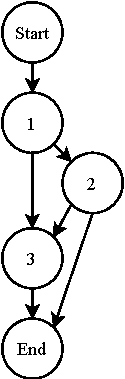
\includegraphics[height=1.5in]{img/Background/control-flow-graph.pdf}
    \label{fig:background_control_flow_graph_image}
    \end{minipage}
&
\begin{minipage}[c]{0.45\textwidth}
\centering
\begin{lstlisting}[language=Python, label=lst:background_control_flow_graph_listing]
def function(a,b):
    if a < b: # (1)
        if b < 10: #(2)
            a = a + b
        else:
            return b #(end)
    a = a * 2 #(3)
    return a #(end)
\end{lstlisting}
\end{minipage}
\end{tabular}
\caption{Control-flow graph visualisation for a code sample. The graph has six edges, five nodes and one connected component. The cyclomatic complexity is 3.}
\label{fig:background_control_flow_graph}
\end{figure}

The cyclomatic complexity on a control-flow graph as the number of linearly independent execution paths is defined as:
\begin{equation}\label{eq:cyclomatic_complexity}
M = E - N + 2P
\end{equation}

$E$ is the number of edges, $N$ the number of nodes and $P$ the number of connected components.  A connected graph is a subgraph, in which all nodes are connected to each other by a path. Following this definition, the cyclomatic complexity can be calculated. \Cref{fig:background_control_flow_graph} shows a visualisation of a sample python function. The control-flow graph has six edges, five nodes and is one connected component. Using \Cref{eq:cyclomatic_complexity}, the cyclomatic complexity is 3.

MacCabe recommends limiting the cyclomatic complexity to 10~\cite{mccabe_complexity_1976}. A lower cyclomatic complexity improves testability since the complexity represents the number of execution paths that need to be tested. Therefore, $M$ is the upper bound for the number of test cases for full branch coverage. 
Software that has to comply with safety standards like ISO 26262 (for electronics in automobiles) or IEC 62304 (for medical devices) are mandated to have a low cyclomatic complexity~\cite{isotc_22sc_32_iso_2018, isotc_210_iec_2006}.

Although cyclomatic complexity is used throughout the industry, several shortcomings are under critique. First, complexity from data flow is ignored. Working with a larger number of variables and operations, the code becomes more complicated, but the cyclomatic complexity does not take this into account. Second, nested code structures are not considered by the metric, although it adds additional difficulty for understanding~\cite{yu_survey_2010}.

\subsection{Halstead Complexity Measures}
Maurice Halstead introduced the Halstead complexity measures (HCM) in 1977~\cite{halstead1977elements}. Halstead approached the complexity measure with an empirical approach by defining observable and measurable properties and put them into relations.

The measurable properties are operators and operands. Operators are symbols in expressions like an addition, subtraction or multiplication symbol. Operands are the values and variables that are manipulated by the operators. 

The sum and number of distinc operators and operands are counted as:
\begin{itemize}
    \item $\eta_1$ as the number of distinct operators 
    \item $\eta_2$ as the number of distinct operands
    \item $N_1$ is the sum of all operators
    \item $N_2$ is the sum of all operands  
\end{itemize}

From these base properties, Halstead derrived additional properties:
\begin{itemize}
    \item Program vocabulary size:
    \begin{displaymath}
        \eta = \eta_1 + \eta_2
    \end{displaymath}
    \item Program length as the sum of all operators and operands:
    \begin{displaymath}
        N = N_1 + N_2
    \end{displaymath}
    \item The volume of a program in terms of program length and program vocabulary is defined as: 
    \begin{displaymath}
        V = N * \log_2{\eta}
    \end{displaymath}
\end{itemize}

Based on those properties, code metrics can be calculated. 
First, the difficulty of understanding a program is calculated as:
\begin{displaymath}
    D = \frac{\eta_1}{2} * \frac{N_2}{\eta2}
\end{displaymath}
The major contributors to difficulty are the number of distinct operators $\eta_1$ and the sum of all operands $N_2$.

Second, the combination of difficulty and volume is the required effort for understanding or changing code follows:
\begin{displaymath}
    E = D * V
\end{displaymath}

Third, the effort for changes translates into real time following the relation:
\begin{displaymath}
    T = \frac{E}{18}s.
\end{displaymath}

Last, the number of bugs correlates with the following relation~\cite{yu_survey_2010}:
\begin{displaymath}
    B = \frac{V}{3000}
\end{displaymath}

HCM focus on the complexity introduced by data manipulation but ignores complexity from the control-flow. Since the cyclomatic complexity focuses on the control-flow complexity but not on the data-flow complexity, it is practical to use both together to supplement each drawback~\cite{yu_survey_2010}.
Additionally, the correlation with the number of bugs is based on the programmer's skill estimation with a fixed value of 3000. Since this varies between projects, such an experiential and fixed number is doubtable~\cite{yu_survey_2010}.

\subsection{Software Maintainability Index}
The software maintainability index was developed by Dan Coleman and Paul Oman in 1994. 16 HP engineers evaluated 16 software systems and scored it in a range from 0 to 100, with 100 representing best maintainability~\cite{coleman_using_1994}. 
Following a regression analysis, they identified the following equation to match the maintainability of the evaluated systems:
\begin{displaymath}
MI = 171 - 5.2 *\ln{\overline{V}} - 0.23 * \overline{M} - 16.2 * \ln{\overline{LOC}} + 50 * \sin{\sqrt{2.4 * C}}
\end{displaymath}
$\overline{V}$ is the average Halstead Volume, $\overline{M}$ the average cyclic complexity, $LOC$ the lines of code and $C$ as fraction of comments.

The software maintainability index was defined many years ago with a limited sample size of developers and projects. Additionally, programming languages have changed significantly over time. A study by Sjøberg et al. suggests no correlation between the software maintainability index and actual maintenance effort in a controlled environment~\cite{sjoberg_questioning_nodate}. Although the study only analyes four software projects and lacks generalization, they found a strong anti-correlation with different maintainability metrics. Only the code size seems to correlate with the actual maintainability. The former seems to be consistent with a systematic review on software maintainability predictions and metrics by Riaz et. al~\cite{riaz_systematic_2009}.

\subsection{Application on Clean Code}
The described metrics are used to quantify the code quality. Since the clean code principles have a positive impact on code quality, lower code quality metrics may indicate more rule violations. The Halstead Metric derives the understandability of different parts of the code but does not explain the reason for it. Similarly, a high cyclomatic complexity of a function can indicate a violation against the recommended single purpose per function. In other words, the metrics indicate parts of code with low quality without pinpointing a specific violation of clean code rules. 


\section{Tools for Code Quality Analysis}\label{sec:tool_comparison}
With quantitative metrics for software quality, different tools can analyse source code and can inform about the increase or decrease in code quality. It is good practice to use static code analysis tools to improve code quality. A static code analysis examines a program by analyzing an abstract syntax tree, the control or data flow, a pointer analysis or an abstract (approximated) execution. In comparison to dynamic analysis, the code is not executed. The result of static analysis can be based on approximations, so there might be false-positive results. An expert has to examine the result if necessary~\cite{prahofer_static_2017}.

Besides the use of static code analysis for compiler and optimizations, it is also helpful for analyzing the code quality. The tools in this chapter analyse different categories of code quality-related principles:
\begin{description}
    \item[Code Guidelines:] A static code analysis can ensure compliance to structural, naming and formatting code guidelines. 
    \item[Standard Compliance:] A requirement for a software may be compliance to an industry-standard like IEC 61508 or ISO 26262~\cite{tc_65sc_65a_iec_2010,isotc_22sc_32_iso_2018}. Static code analysis can ensure or at least assist with the compliance.  
    \item[Code Smells:] Some code smells follow a known pattern and a static code analysis can detect those smells. Since code smells can be an indication for chaotic code, it is best if these smells are detected and removed early on.
    \item[Bug Detection:] Although bug detection with static analysis can not detect all bugs, every detected bug before a software release is essential. Examples for detected bugs are unhandled expressions or concurrency issues~\cite{delaitre_evaluating_2015}.
    \item[Security Vulnerability Detection:] Static code analysis tools can detect some security vulnerabilities like SQL Injection Flaws, buffer overflows and missing input validation with high confidence. Since these are some common, easy to exploit vulnerabilities, an analysis for security vulnerabilities can increase the security of the overall software~\cite{wichers_source_nodate}.  
\end{description}

The categories of code guidelines and code smells can be used to detect un-clean code.

The following sections provide an overview of several static code analysis tools with a focus on code quality and maintainability. We selected them based on popularity and if the projects are still maintained.

\subsection{PyLint}
PyLint is a code analysis tool for the Python programming language. It is open-source and licensed under the GNU General Public License v2.0 and available for all common platforms. PyLint can be executed as a standalone program or can be integrated into common IDEs like Eclipse. A continuous integration pipeline may include PyLint as well to ensure an analysis on every build.

With PyLint, the developer can make sure that the code complies to the PEP 8 style guide for python coding~\cite{pep8}. This includes name formatting, line length and more. It does not calculate a metric for the code but instead warns about violated principles. Additionally, PyLint can detect common errors like missing import statements that may cause the program to crash at the start or later at runtime. To support refactoring, PyLint can detect duplicated code and will suggest refactoring the code.

PyLint can be configured to ignore some checks and to disable specific rules. To expand the ruleset, a developer can write a "checker", an algorithm to check for a specific rule. The algorithm can analyse the raw file content, a token stream of the source code or an AST representation. The checker can raise a rule violation by providing the location information and the problem type to the PyLint framework, and it can be included in the PyLint analysis report. TODO pylint cite

\subsection{PMD Source Code Analyzer Project}
PMD is an "extensible cross-language static code analyzer"~\cite{noauthor_pmd_nodate} for Java, JavaScript and more. As an open-source project, it is licensed under a BSD-style license and is available for macOS, Linux and Windows-based systems. It integrates into build systems like Maven and Gradle as well as into common IDEs like Eclipse and IntelliJ. PMD can run as part of a continuous integration pipeline and is included in the automated code review tool Codacy~\cite{noauthor_codacy_nodate-1}.

Depending on the target language, PMD supports different rules. For Java, PMD has rules in the following categories~\cite{noauthor_documentation_nodate}.
\begin{description}
    \item[Best practices:] Best practices include rules like one declaration per line or using a logger instead of a \textit{System.out.print()} in production systems.  
    \item[Coding Style and Design] Several rules to improve the readability of the code like naming conventions, ordering of declarations and design problems like a violation of the Law of Demeter, Cyclomatic complexity calculation and detection of god classes.
    \item[Multithreading :]  Rules to mainly prevent the use of not thread-safe objects or methods. Due to the nature of multithreading and unpredictable scheduling of threads, problems like unpredictable values of variables or deadlocks may occur. Since they may not occur in every execution, they are hard to spot and to debug. Consequently, warnings of using non-thread-safe code may save hours of debugging.
    \item[Performance:] These rules flag known operations that have hidden performance implications. For example, string concatenation with the plus operator in Java causes the Java Virtual Machine to create an internal string buffer. This can slow down the program execution if numerous string concatenations are performed.
    \item[Security:] Security-wise, PMD only checks for hardcoded values for cryptographic operations like keys and initialization vectors.
    \item[Error Prone Code:] PMD checks for several known code structures that will or may cause a bug at execution. Some rules are part of the clean code principles described in \Cref{sec:clean_code}, and some rules are specific to the target language.
\end{description}

A user can expand the PMD ruleset in two ways: A XPath expression can be specified and will be validated against the AST by the PMD framework. For more control, it is possible to write a Java-based plugin that implements a custom AST traverser. The latter allows for more sophisticated rules and checks~\cite{noauthor_documentation_nodate}.

\subsection{Codacy}
Codacy is a software to "check your code quality"~\cite{noauthor_codacy_nodate} for more than 30 programming languages. It is available as a cloud-based subscription service with a free tier for open-source projects and a self-host option for enterprise customers.  Codacy runs as cloud software, and a user can connect a GitHub, GitLab or Bitbucket repository that will be scanned automatically on every push or trigger a scan of local files with a command-line program. Additionally, a badge can be added to the readme page to show off the analysis results.

Codacy can be seen as a platform that runs multiple different "analysis engines". These analysis engines combine multiple tools depending on the language. For Python, Codacy uses  PyLint, Bandit (a scanner for security issues) and a metric plugin.
Due to the licensing of those analysis engines, the engines are open-sourced, whereas the Codacy platform is proprietary.

Depending on the language, Codacy supports scanning for common security and maintainability issues. The later is faced with scanning for Code Standardization, Test Coverage and Code Smells to reduce technical debt.

Codacy allows customization by disabling specific rules and changing rule parameters like the pattern to fit the rules to the project~\cite{noauthor_codacy_nodate}. 

\subsection{Sonarqube}
Sonarqube is an analysis tool to maintain high code quality and security. It supports 15 programming languages in the open-source version licensed under the GNU Lesser General Public License, Version 3.0. In the Developer Edition, Sonarqube supports 22 languages and 27 languages in the enterprise edition. Sonarqube is a self-hostable server application with a SonarScanner client module that can be integrated into build pipelines like Gradle and Maven as well as a command-line tool for other build pipelines. The SonarScanner reports the result to the server, that serves a website to review the results. With the Developer Edition, branch and pull request analysis are possible, and a pull request will be annotated with the analysis results~\cite{noauthor_code_nodate}.

For Python, Sonarqube offers more than 170 rules. These rules are in the following categories~\cite{noauthor_python_nodate}:
\begin{description}
    \item[Code Smells:] Code Smells like duplicated String literals are flagged with four different levels of severity (from higher to lower severity): Blocker, Critical, Major, Minor. Explanations and examples are accessible for the developer to understand and fix the issue. The analysis is more in-depth than AST-based solutions since it additionally uses control and data flow analysis.
    \item[Bug:] Multiple rules cover bugs that would definitively result in a runtime exception and program termination. As an example, calling a function with the wrong number of arguments will be flagged with the highest severity, since it will raise a TypeError during runtime. Although programmers may notice issues like this during coding and testing, the issue can remain hidden if it is only triggered by a particular execution path of the system.
     \item[Security Hotspot:] The Security Hotspot analysis unfolds pieces of code that may be a real vulnerability and requires a human review. The scanning has a hotspot detection for seven out of the OWASP Top Ten Web Application security risks~\cite{noauthor_python_nodate}. A flagged hotspot contains a detailed explanation of the reason for being flagged and a guide on how to review this hotspot. The recommendation to double-check a piece of code can help to prevent a security vulnerability from being deployed to production.
    \item[Security Vulnerabilities:]  A security vulnerability analysis reveals a code that is at risk of being exploited and has to be fixed immediately. For example, misconfigurations of cryptographic libraries can be revealed quickly, and possible damage can be proactively prevented.   
\end{description}

Additionally, Sonarqube offers several metrics like test coverage and a custom derivate of Cyclomatic Complexity named Cognitive Complexity~\cite{campbell2018cognitive}. The authors see several shortcomings in the original Cyclomatic Complexity model:
\begin{itemize}
    \item Parts of code with the same Cyclomatic Complexity do not necessarily represent an equal difficulty for maintenance.
    \item  Cyclomatic Complexity does not include modern language features like try/catch and lambdas. Therefore, the score can not be accurate anymore.
    \item Cyclomatic Complexity lacks useability on a class or module level. Small class with complex methods would have the same Cyclomatic Complexity as large classes with low complexity per method (such as getter or setter methods). The informative value of the metric is low.
\end{itemize}
Cognitive Complexity addresses these points, especially the incorporation of modern language features and meaningfulness on class and module level.

The calculation is based on three rules~\cite{campbell2018cognitive}:
\begin{description}
    \item[Ignore Shorthand Structures]: Method calls condense multiple statements into one easy-to-understand statement. Therefore, method calls as shorthand are ignored for the score. Similarly, shorthand structures like the null-coalescing operator reduce the Cognitive Complexity compared to an extensive null check and are therefore ignored for score calculation.
    \item[Break in the linear control flow]: A break in the expected linear control flow by loop structures and conditionals adds to Cognitive Complexity as well as to Cyclomatic Complexity. Additionally, catches, switches, sequences of logical operators, recursion, and jumps also adds to Cognitive Complexity, since these structures break the linear control flow.
    \item[Nested flow-breaking strcutures]: Flow-breaking structures that are nested additionally increase the Cognitive Complexity, since it is harder to understand than non-nested structures.  
\end{description}
The method-level Cognitive Complexity score represents a relative complexity difference between methods that would have the same Cyclomatic Complexity. Furthermore, the aggregated Cognitive Complexity on a class or module level differentiates between classes with many, simple methods and classes with a few, but complex methods. As a result, domain classes (containing mainly getters/setters) have a lower score compared to classes with complex code behaviour~\cite{campbell2018cognitive}.

Developers can extend Sonarqube similarly to PMD. They can write a Java plugin that can access the AST but also a semantic model of the code. Additional, extensions can be created that provide the functionality to other extensions. The Java plugin is compiled into a \texttt{.jar} file and placed into the plugin dir of the Sonarqube installation. For more straightforward rules, XPath expressions are possible through the web interface and allow a quick extension. For instance, if developers observe bad code style during a pull request review, they can quickly write a rule to enforce this rule in all subsequent pull requests automatically.

\section{Automated Detection of Clean Code Violations}
We described the background and related work to different aspects of code quality, such as quality metrics (in \Cref{sec:cyclomatic_complexity}) and tools that detect problems in code (in \Cref{sec:tool_comparison}). Those tools can help to improve the code quality and detect code smells. Code smells can be an indicator of clean code violations. Several studies have been performed to improve the code smell detection: Fernandes et al. compare 84 tools to detect code smell (TODO cite A Review-based Comparative Study of Bad Smell Detection Tools Eduardo Fernandes, Johnatan Oliveira, Gustavo Vale, Thanis Paiva, Eduardo Figueiredo ) and Fontana et al. (TODO cite Comparing and experimenting machine learning techniques for code smell detection) apply 16 machine learning models on code smells by using quantitative metrics as model input. A recent literature review by Azeem et al. ((TODO cite Machine learning techniques for code smell detection: A systematic literature review and meta-analysis)) compares studies for machine learning for code smell detection and that most models use quantitative metrics as features. Their results indicate an \enquote{absence of studies investigating metrics different from the structural
ones}TODO cite as before).

We do not want to detect code smells but directly identify clean code violations on a source code level. Code smells can indicate clean code violation, but they do not necessarily pinpoint the root cause of the problem. A code smell that indicates a long function violates the clean code rule of small functions but does point to problems such as mixing different abstraction level. Additionally, we want to utilise the source code as a feature set directly without extracting higher-level metrics.